\subsection{Failure Analysis}


\begin{figure}[t]
    \centering
    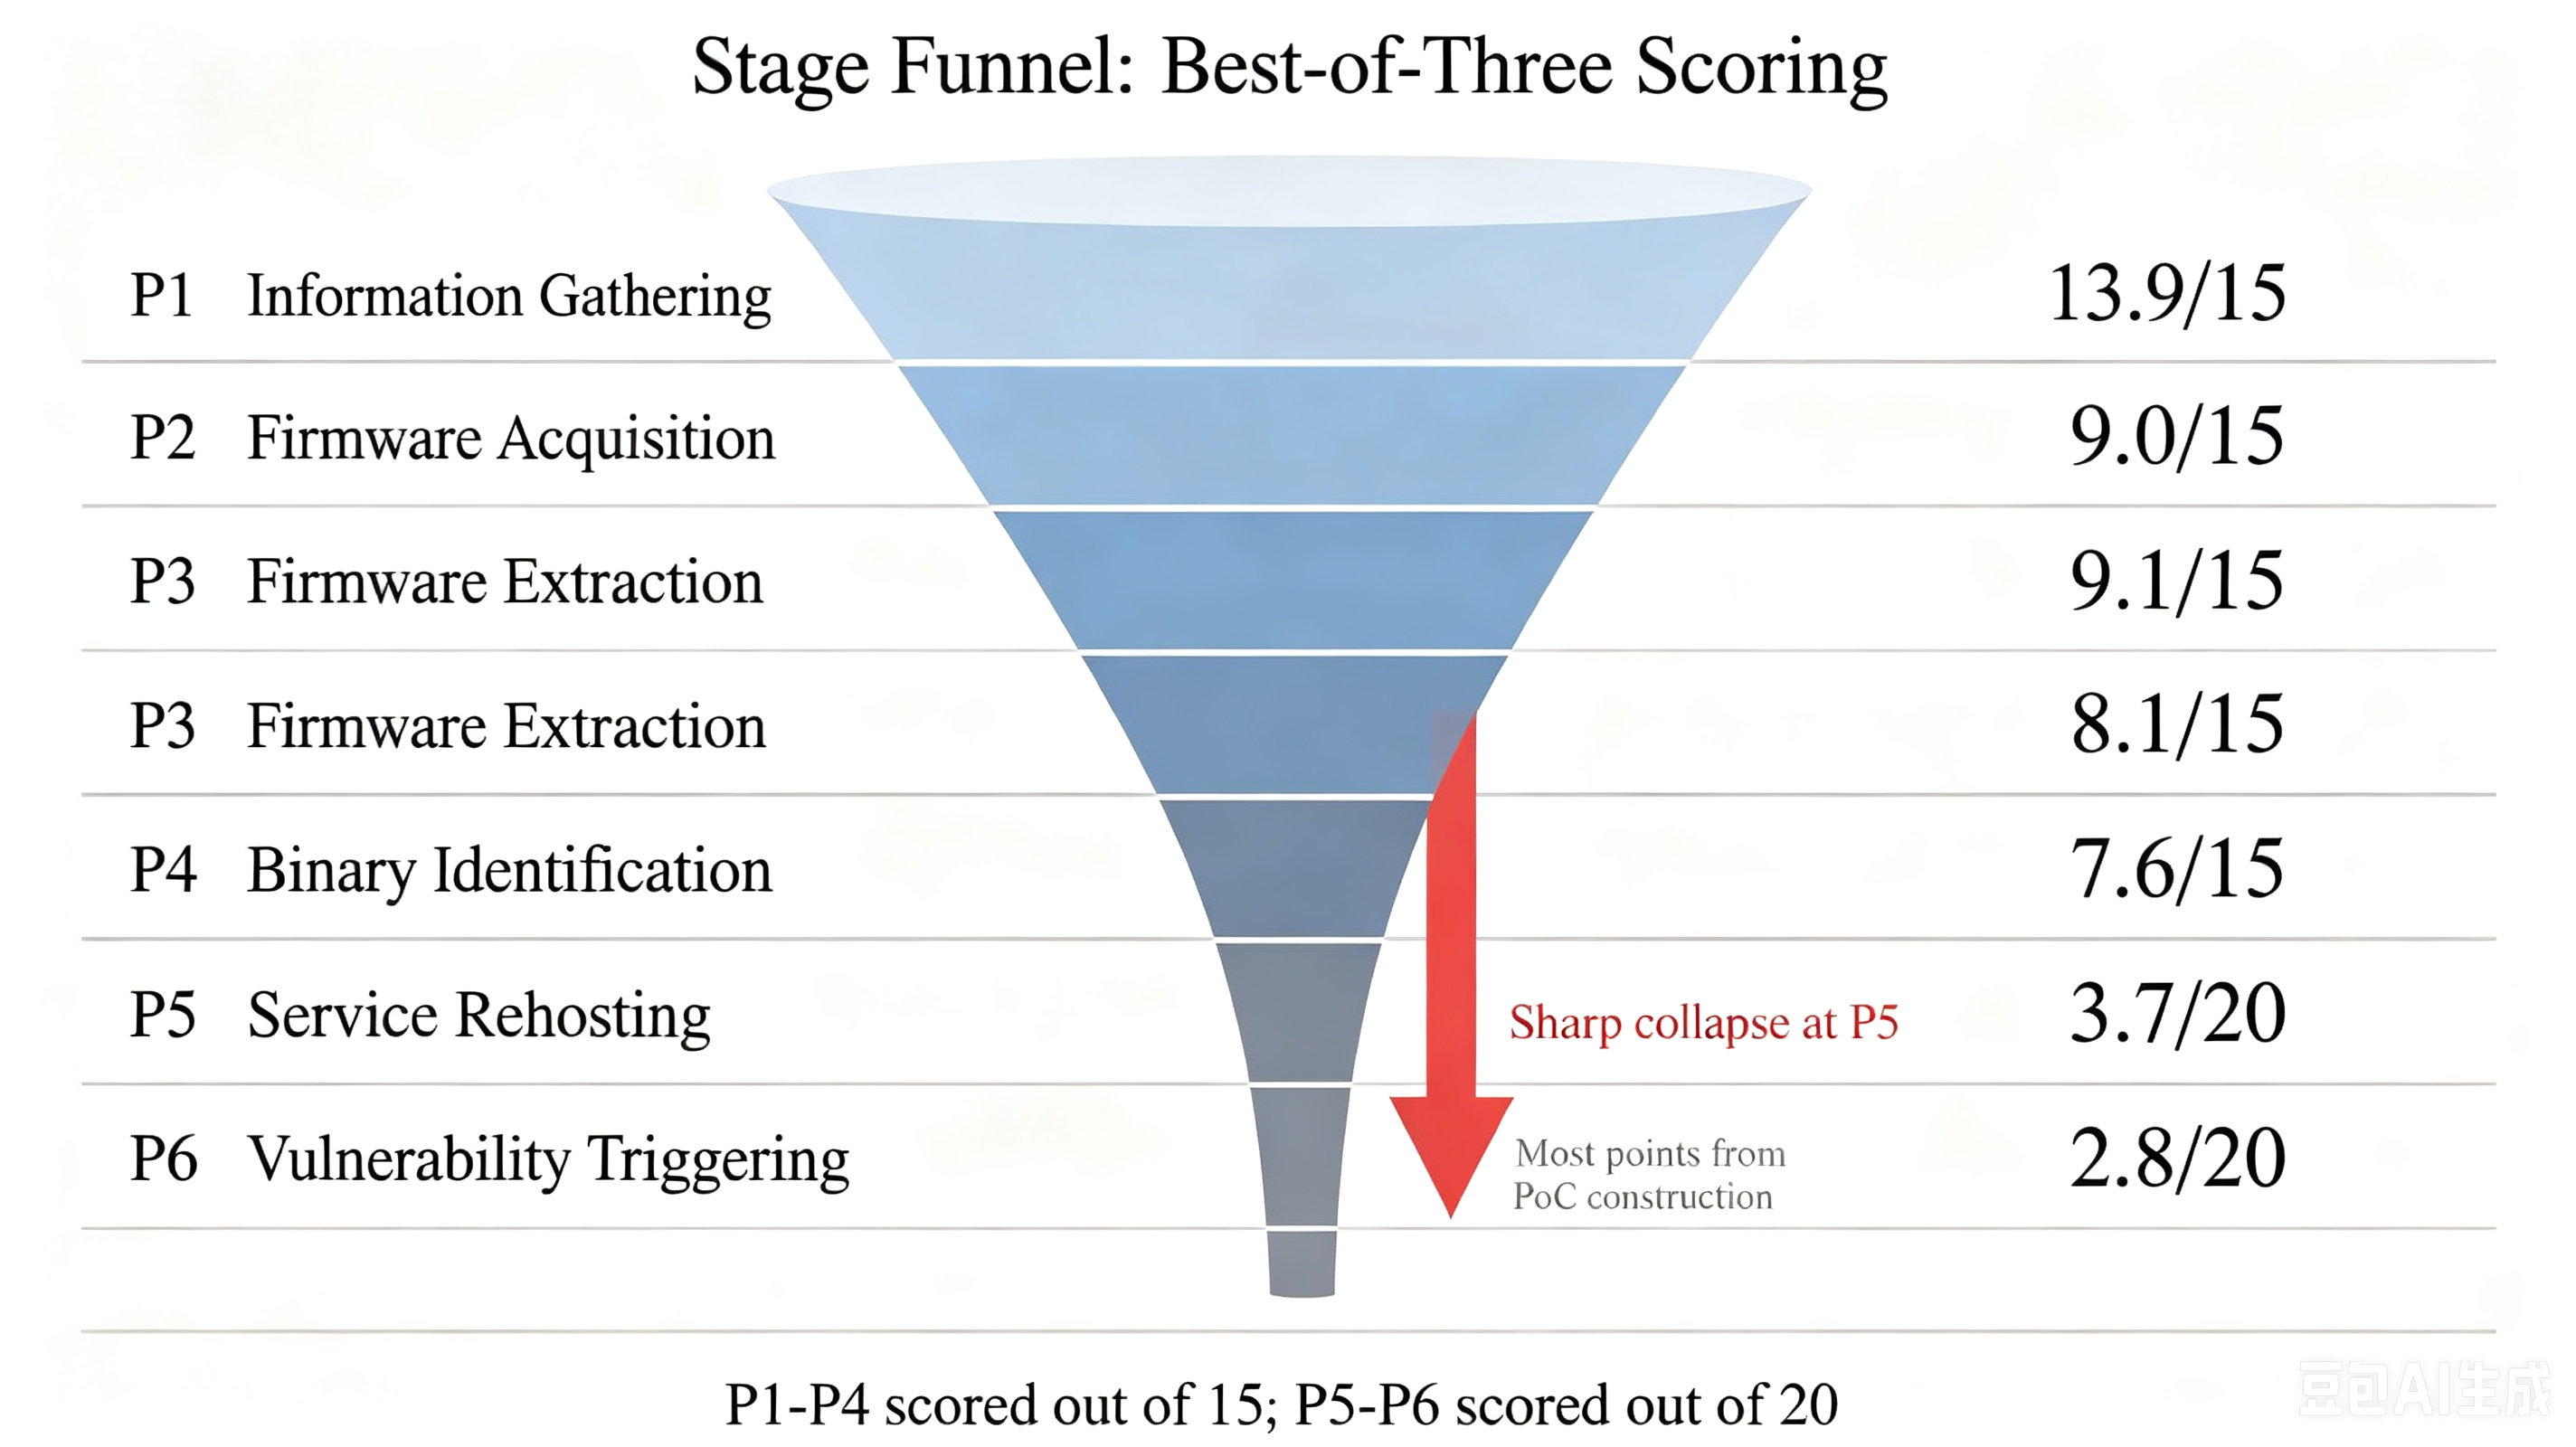
\includegraphics[width=0.47\textwidth]{figures/stage-funnel.png}
    \caption{Stage-level averages under best-of-three scoring.}
    \label{fig:stage-funnel}
\end{figure}


% RQ2: 阶段漏斗——P1-R4合理，R5骤降，terminal blocker主要在Phase 5
Figure~\ref{fig:stage-funnel} shows the stage funnel from P1 to P6. P1 (Information Gathering) is the strongest phase at 13.9/15, indicating that most agents successfully collect CVE facts. P2--P4 show moderate scores (7.6--9.0/15), reflecting partial success in firmware acquisition, extraction, and binary identification. The sharp collapse occurs at P5 (Service Rehosting), which averages only 3.7/20. P6 averages 2.8/20, with most points coming from PoC construction rather than real-target triggering.

%%\begin{table}[t]
%%\setlength{\tabcolsep}{3.8pt}
%%\centering
%%\caption{Stage-level averages under %%best-of-three scoring. The pipeline %%collapses at P5.}
%%\label{tab:stage-funnel}
%%\renewcommand{\arraystretch}{1.15}
%%\begin{tabular}{c l r r r}
%%\toprule
%%\textbf{Phase} & \textbf%%{Description} & \textbf{Score} & %%\textbf{Max} & \textbf{\%} \\
%%\midrule
%%P1 & Information gathering   & 13.%%9 & 15 & 92.8\% \\
%%P2 & Firmware acquisition    &  9.%%0 & 15 & 59.8\% \\
%%P3 & Firmware extraction     &  8.%%1 & 15 & 53.7\% \\
%%P4 & Binary identification   &  7.%%6 & 15 & 50.8\% \\
%%\midrule
%%P5 & Service rehosting       &  3.%%7 & 20 & 18.6\% \\
%%P6 & Vulnerability triggering&  2.%%8 & 20 & 13.8\% \\
%%\bottomrule
%%\end{tabular}
%%\end{table}



Across all 450 runs, terminal blockers fall into four failure families, ordered below by descending frequency, and cluster at two phases---P2 (202/450) and P5 (109/450)---consistent with the funnel above. The dominant families are reproduction-logic errors; a small residual involves the execution environment.

\noindent{\textbf{Simulation substitution (316/450, 70.2\%).}} The dominant failure: agents produce mock servers, C harnesses, or host-native programs that demonstrate the vulnerability \emph{pattern} but not the target \emph{instance}. The output is often coherent and reproducible---valid crash signals, correct exploit syntax, convincing reports---yet never exercises the real firmware binary, so real-target gating rejects all of these.

\noindent{\textbf{Rehosting gap (97/450, 21.6\%).}} Agents identify the target binary but cannot configure dynamic loaders, NVRAM values, or network listeners under QEMU, and abandon after one or two errors. Same-architecture (ARM64) devices bypass this gap via \texttt{chroot}, leaving cross-architecture (MIPS) targets that require QEMU emulation as the bulk of these blockers.

\noindent{\textbf{Extraction failures (37/450, 8.2\%).}} Agents acquire firmware but misuse extraction tools---e.g., applying standard \texttt{binwalk} to vendor-encrypted images---or analyze binaries pulled from PoC repositories rather than from the target firmware.

\noindent{\textbf{Infrastructure failures (15/450, 3.3\%).}} The residual blockers stem from execution-environment setup rather than reproduction logic, and are scattered across phases rather than concentrated at any single stage.
